%==============================================================
%  EE201 -- Circuit Theory I
%  Lecture 4 : The Capacitor -- slides
%  M. Mert Ankaralı, METU EEE
%
%  Compile:  ./build.sh      (or: pdflatex EE201_Lecture_4_slides.tex, twice)
%  Same colour code as the handout:
%      charge = purple, current = blue, voltage = orange, power = green
%==============================================================
\documentclass[11pt,aspectratio=169]{beamer}

\usepackage[T1]{fontenc}
\usepackage[utf8]{inputenc}
\usepackage[english]{babel}
\usepackage{lmodern}
\usepackage{amsmath,amssymb}
\usepackage{booktabs}
\usepackage{array}
\usepackage{colortbl}
\usepackage{tikz}
\usepackage[american,siunitx]{circuitikz}
\usetikzlibrary{arrows.meta,positioning,calc,decorations.pathreplacing,decorations.pathmorphing,decorations.markings}
\usetikzlibrary{overlay-beamer-styles}

%-------------------- plain METU-flavoured theme --------------
\usetheme{default}
\usecolortheme{default}
\useinnertheme{rectangles}
\setbeamertemplate{navigation symbols}{}
\setbeamertemplate{itemize items}[square]
\setbeamerfont{frametitle}{size=\large,series=\bfseries}
\setbeamerfont{title}{size=\LARGE,series=\bfseries}

\definecolor{metured}{RGB}{155,27,48}
\definecolor{metugray}{RGB}{88,89,91}
\definecolor{metulight}{RGB}{243,240,241}
\definecolor{ccur}{RGB}{0,102,170}
\definecolor{cvolt}{RGB}{214,120,0}
\definecolor{cpow}{RGB}{23,128,74}
\definecolor{ccharge}{RGB}{124,60,160}

\setbeamercolor{structure}{fg=metured}
\setbeamercolor{frametitle}{fg=metured,bg=}
\setbeamercolor{title}{fg=metured}
\setbeamercolor{normal text}{fg=black!88}
\setbeamercolor{block title}{fg=white,bg=metured}
\setbeamercolor{block body}{bg=metulight}
\setbeamercolor{alerted text}{fg=metured}

\setbeamertemplate{frametitle}{%
  \vspace{0.55em}%
  \usebeamerfont{frametitle}\usebeamercolor[fg]{frametitle}\insertframetitle\par
  \vspace{-0.2em}{\color{metured}\rule{\textwidth}{1pt}}\par\vspace{-0.2em}}

\setbeamertemplate{footline}{%
  \hbox{\begin{beamercolorbox}[wd=\paperwidth,ht=2.4ex,dp=1.4ex,leftskip=1.2em,rightskip=1.2em]{}%
  \tiny\color{metugray}\coursecode\ \textbar\ Lecture 4: The Capacitor
  \hfill \insertframenumber/\inserttotalframenumber
  \end{beamercolorbox}}}

%-------------------- macros ----------------------------------
\newcommand{\coursecode}{EE201}
\newcommand{\term}{Fall 2026--2027}
\newcommand{\Icol}[1]{\textcolor{ccur}{#1}}
\newcommand{\Vcol}[1]{\textcolor{cvolt}{#1}}
\newcommand{\Pcol}[1]{\textcolor{cpow}{#1}}
\newcommand{\Qcol}[1]{\textcolor{ccharge}{#1}}
\newcommand{\uni}[1]{\,\mathrm{#1}}
\newcommand{\A}{\uni{A}} \newcommand{\V}{\uni{V}}
\newcommand{\W}{\uni{W}} \newcommand{\J}{\uni{J}}
\newcommand{\Cb}{\uni{C}} \newcommand{\s}{\uni{s}}

\ctikzset{bipoles/length=0.9cm, label/align=straight,
          bipoles/vsourceam/height=0.85, bipoles/vsourceam/width=0.85}
\tikzset{
  curarr/.style={-{Stealth[length=2.6mm]}, ccur, very thick},
  blk/.style={draw=metugray, fill=metulight, rounded corners=2pt,
              minimum height=1.25cm, text width=2.45cm, align=center, font=\scriptsize},
  flowarr/.style={-{Stealth[length=3mm]}, metured, very thick},
  thru/.style={-{Stealth[length=2.2mm]}, ccur, very thick},
  acr/.style={{Stealth[length=2mm]}-{Stealth[length=2mm]}, cvolt, very thick},
  pan/.style={draw=gray!35, fill=metulight, rounded corners=3pt,
              minimum width=3.0cm, minimum height=2.3cm},
  pcap/.style={font=\scriptsize\bfseries, text=metured},
  pol/.style={font=\small, text=cvolt},
  iar/.style={-{Stealth[length=2.4mm]}, ccur, very thick},
  gnode/.style={circle, fill=metured, inner sep=0pt, minimum size=4.2pt},
  glab/.style={font=\footnotesize, text=metured},
  surf/.style={draw=cpow, very thick, dashed, rounded corners=6pt},
  gbr/.style={metugray, thick, postaction={decorate, decoration={markings,
      mark=at position 0.58 with {\arrow{Stealth[length=2.4mm]}}}}},
  vax/.style={-{Stealth[length=2mm]}, gray!70},
  crv/.style={metured, very thick},
  ttl/.style={font=\scriptsize\bfseries, text=metugray},
}

\newcommand{\ohm}{\,\Omega}
\newcommand{\Req}{R_{\mathrm{eq}}}
\newcommand{\viaxes}[3]{%
  \draw[vax] (-#1,0) -- (#1,0) node[right=1pt, font=\scriptsize, text=cvolt] {$v$};
  \draw[vax] (0,-#2) -- (0,#2) node[above=1pt, font=\scriptsize, text=ccur] {$i$};
  \node[ttl] at (0,-#2-0.68) {#3};}
\newcommand{\qvaxes}[3]{%
  \draw[vax] (-#1,0) -- (#1,0) node[right=1pt, font=\scriptsize, text=cvolt] {$v$};
  \draw[vax] (0,-#2) -- (0,#2) node[above=1pt, font=\scriptsize, text=ccharge] {$q$};
  \node[ttl] at (0,-#2-0.68) {#3};}
\newcommand{\taxes}[4]{%
  \draw[vax] (-0.15,0) -- (#1,0) node[right=1pt, font=\scriptsize] {$t$};
  \draw[vax] (0,-#2) -- (0,#3) node[above=1pt, font=\scriptsize] {#4};}

\hypersetup{colorlinks=true,allcolors=metured}

\title{Lecture 4: The Capacitor}\subtitle{an ideal energy-storage element --- and the first that remembers}
\author{M. Mert Ankaralı}
\institute{\small Department of Electrical and Electronics Engineering\\
           Middle East Technical University}
\date{}



%==============================================================
\begin{document}

%--------------------------------------------------------------
\begin{frame}[plain]
  \titlepage
  \vspace{-1.2em}
  \begin{center}\scriptsize\color{metugray}
    \Qcol{$\blacksquare$}~charge \quad \Icol{$\blacksquare$}~current \quad
    \Vcol{$\blacksquare$}~voltage \quad \Pcol{$\blacksquare$}~power, energy
  \end{center}
\end{frame}

%--------------------------------------------------------------
\begin{frame}{An element that stores energy}
  \vfill
  \begin{center}
  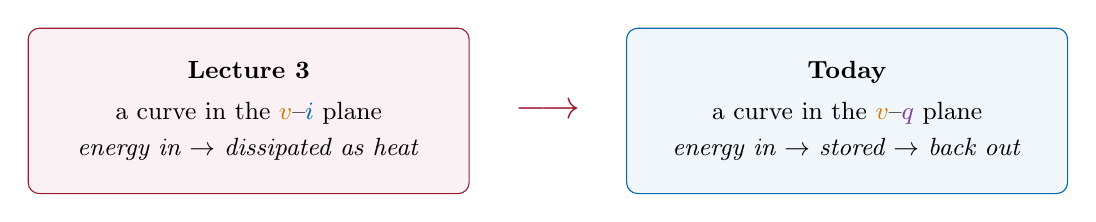
\begin{tikzpicture}[scale=1.0]
    \node[draw=metured, fill=metured!6, rounded corners=4pt, minimum width=5.6cm,
          minimum height=2.1cm, align=center, font=\small] (a) at (0,0)
         {\textbf{Lecture 3}\\[4pt] a curve in the $\Vcol{v}$--$\Icol{i}$ plane\\[2pt]
          \emph{energy in $\to$ dissipated as heat}};
    \node[draw=ccur, fill=ccur!6, rounded corners=4pt, minimum width=5.6cm,
          minimum height=2.1cm, align=center, font=\small] (b) at (7.6,0)
         {\textbf{Today}\\[4pt] a curve in the $\Vcol{v}$--$\Qcol{q}$ plane\\[2pt]
          \emph{energy in $\to$ stored $\to$ back out}};
    \node[font=\Large, text=metured] at (3.8,0) {$\longrightarrow$};
  \end{tikzpicture}
  \end{center}
  \vfill
  \begin{center}
    A resistor \alert{dissipates}: $\Pcol{p} = R\Icol{i}^2 \ge 0$ always, so the energy
    it is given turns into heat and never comes back.\\[6pt]
    {\large Today's element dissipates nothing. It is an \alert{ideal energy-storage
     element} --- everything put in can be taken back out, which is also why it
     \alert{remembers}.}
  \end{center}
  \vfill
\end{frame}

%--------------------------------------------------------------
\begin{frame}{Every domain has one}
  \vfill
  \begin{center}
  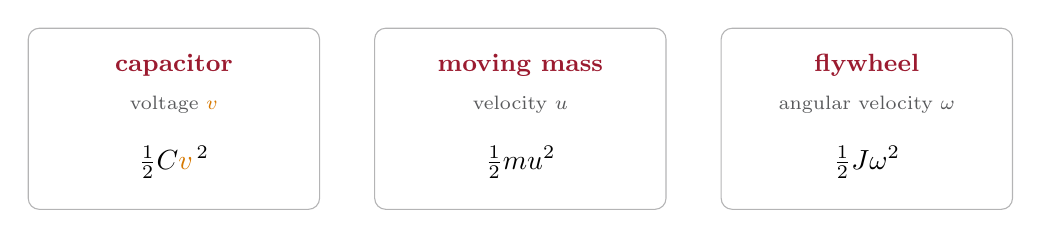
\begin{tikzpicture}[scale=1.0]
    \foreach \dx/\ttl/\sub/\expr in {0/{capacitor}/{voltage $\Vcol{v}$}/{$\tfrac12 C\Vcol{v}^{\,2}$},
                                4.4/{moving mass}/{velocity $u$}/{$\tfrac12 m u^2$},
                                8.8/{flywheel}/{angular velocity $\omega$}/{$\tfrac12 J\omega^2$}}{
      \begin{scope}[xshift=\dx cm]
        \draw[metugray!45, rounded corners=4pt] (-1.85,-1.15) rectangle (1.85,1.15);
        \node[font=\small\bfseries, text=metured] at (0,0.68) {\ttl};
        \node[font=\scriptsize, text=metugray] at (0,0.18) {\sub};
        \node[font=\normalsize] at (0,-0.55) {\expr};
      \end{scope}}
  \end{tikzpicture}
  \end{center}
  \vfill
  \begin{center}
    Charge is electrical bookkeeping. \alert{Energy} is what every domain shares ---
    Lecture~1's table, read one level higher.\\[4pt]
    Each holds half a constant times the square of one variable, and gives all of it
    back.\\[6pt]
    {\small The resistor's mechanical counterpart is \emph{viscous friction}.}
  \end{center}
  \vfill
\end{frame}

%--------------------------------------------------------------
\begin{frame}{Some elements store charge}
  \vfill
  \begin{center}
    {\large For those, the useful pair is not $(\Vcol{v},\Icol{i})$ but
     $(\Vcol{v},\Qcol{q})$.}
  \end{center}
  \vfill
  \begin{center}
    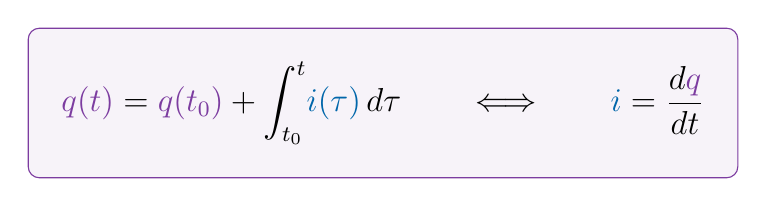
\begin{tikzpicture}
      \node[draw=ccharge, fill=ccharge!6, rounded corners=4pt, inner sep=12pt]
      {\large $\displaystyle \Qcol{q(t)} = \Qcol{q(t_0)} + \int_{t_0}^{t}\!\Icol{i(\tau)}\,d\tau
        \qquad\Longleftrightarrow\qquad \Icol{i} = \frac{d\Qcol{q}}{dt}$};
    \end{tikzpicture}
  \end{center}
  \vfill
  \begin{center}
    $\Qcol{q}$ is the charge that has entered the $+$ terminal. \\
    {\small The link between the two is Lecture 1, unchanged.}
  \end{center}
  \vfill
\end{frame}

%--------------------------------------------------------------
\begin{frame}{What a capacitor is}
  \vfill
  \begin{center}
    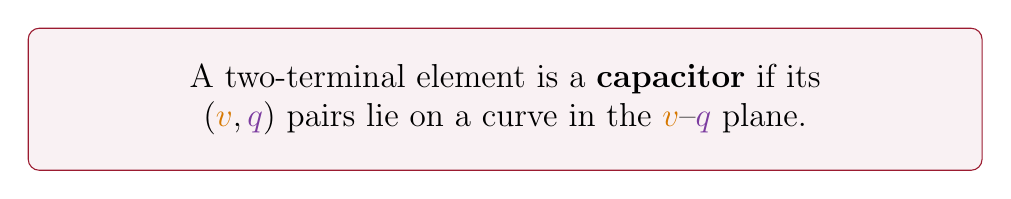
\begin{tikzpicture}
      \node[draw=metured, fill=metured!6, rounded corners=4pt, inner sep=13pt,
            text width=11.2cm, align=center, font=\large]
      {A two-terminal element is a \textbf{capacitor} if its $(\Vcol{v},\Qcol{q})$ pairs
       lie on a \alert{curve in the $\Vcol{v}$--$\Qcol{q}$ plane}.};
    \end{tikzpicture}
  \end{center}
  \vfill
  \begin{center}
  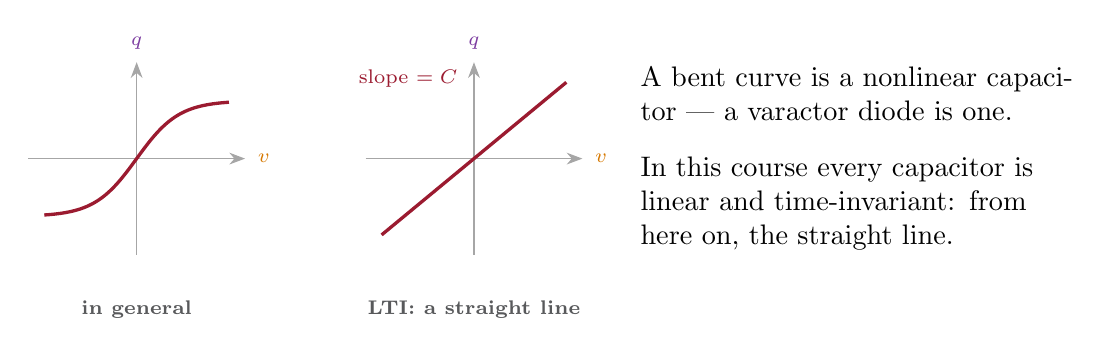
\begin{tikzpicture}[scale=1.02, transform shape]
    \begin{scope}
      \qvaxes{1.35}{1.2}{in general}
      \draw[crv, domain=-1.15:1.15, samples=140, smooth] plot (\x, {0.72*tanh(1.9*\x)});
    \end{scope}
    \begin{scope}[xshift=4.2cm]
      \qvaxes{1.35}{1.2}{LTI: a straight line}
      \draw[crv] (-1.15,-0.95) -- (1.15,0.95);
      \node[font=\scriptsize, text=metured] at (-0.82,1.0) {slope $=C$};
    \end{scope}
    \node[font=\normalsize, anchor=west, text width=5.5cm] at (6.15,0)
      {A bent curve is a nonlinear capacitor --- a varactor diode is one.\\[8pt]
       In this course every capacitor is \alert{linear and time-invariant}: from here on,
       the straight line.};
  \end{tikzpicture}
  \end{center}
  \vfill
\end{frame}

%--------------------------------------------------------------
\begin{frame}{And note what has \emph{not} happened}
  \vfill
  \begin{center}
    {\large A capacitor has \alert{no characteristic} in the
     $\Vcol{v}$--$\Icol{i}$ plane.}\\[4pt]
    {\small There \emph{is} a relation between $\Vcol{v}$ and $\Icol{i}$ --- but not
     between their values at one instant.}
  \end{center}
  \vfill
  \begin{center}
  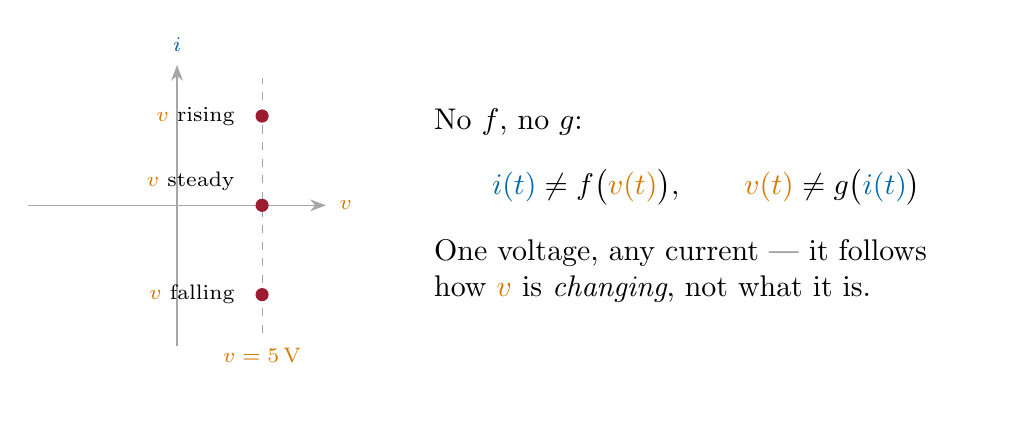
\begin{tikzpicture}[scale=1.08, transform shape]
    \viaxes{1.75}{1.65}{}
    \draw[metugray!55, dashed] (1.0,-1.5) -- (1.0,1.5);
    \node[font=\scriptsize, text=cvolt, below] at (1.0,-1.56) {$\Vcol{v} = 5\V$};
    \fill[metured] (1.0,1.05) circle (2.2pt);
    \fill[metured] (1.0,0) circle (2.2pt);
    \fill[metured] (1.0,-1.05) circle (2.2pt);
    \node[font=\scriptsize, anchor=east] at (0.80,1.05) {$\Vcol{v}$ rising};
    \node[font=\scriptsize, anchor=east] at (0.80,0.28) {$\Vcol{v}$ steady};
    \node[font=\scriptsize, anchor=east] at (0.80,-1.05) {$\Vcol{v}$ falling};
    \node[font=\normalsize, anchor=west, text width=6.4cm] at (2.9,0)
      {No $f$, no $g$:
       \[ \Icol{i(t)} \neq f\bigl(\Vcol{v(t)}\bigr), \qquad
          \Vcol{v(t)} \neq g\bigl(\Icol{i(t)}\bigr) \]
       One voltage, \alert{any} current --- it follows how $\Vcol{v}$ is
       \emph{changing}, not what it is.};
  \end{tikzpicture}
  \end{center}
  \vfill
\end{frame}

%--------------------------------------------------------------
\begin{frame}{Where the charge sits}
  \vfill
  \begin{center}
  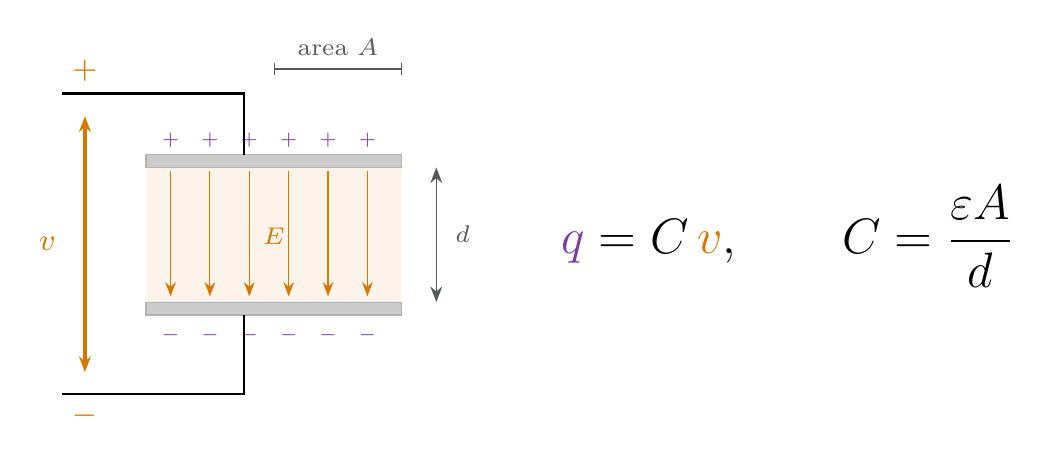
\begin{tikzpicture}[scale=1.25, transform shape]
    \fill[gray!40] (0,0) rectangle (2.6,0.13);
    \fill[gray!40] (0,1.5) rectangle (2.6,1.63);
    \fill[cvolt!8] (0,0.13) rectangle (2.6,1.5);
    \draw[gray!60] (0,0) rectangle (2.6,0.13);
    \draw[gray!60] (0,1.5) rectangle (2.6,1.63);
    \foreach \x in {0.25,0.65,1.05,1.45,1.85,2.25}{
      \draw[cvolt, -{Stealth[length=1.8mm]}, visible on=<2->] (\x,1.46) -- (\x,0.19);
      \node[font=\tiny, text=ccharge] at (\x,1.78) {$+$};
      \node[font=\tiny, text=ccharge] at (\x,-0.2) {$-$};}
    \node[font=\scriptsize, text=cvolt, visible on=<2->] at (1.3,0.8) {$E$};
    \draw[{Stealth[length=2mm]}-{Stealth[length=2mm]}, metugray] (2.95,0.13) -- (2.95,1.5);
    \node[font=\scriptsize, text=metugray, right=2pt] at (2.95,0.82) {$d$};
    \draw[metugray, |-|] (1.3,2.5) -- (2.6,2.5);
    \node[font=\scriptsize, text=metugray, above] at (1.95,2.51) {area $A$};
    \draw[thick] (1.0,1.63) -- (1.0,2.25) -- (-0.85,2.25);
    \draw[thick] (1.0,0) -- (1.0,-0.8) -- (-0.85,-0.8);
    \node[pol] at (-0.62,2.48) {$+$}; \node[pol] at (-0.62,-1.02) {$-$};
    \draw[{Stealth[length=2mm]}-{Stealth[length=2mm]}, cvolt, very thick] (-0.62,-0.58) -- (-0.62,2.02);
    \node[pol] at (-1.0,0.72) {$v$};
    \node[font=\Large, anchor=west, visible on=<3->] at (4.1,0.8)
      {$\displaystyle \Qcol{q} = C\,\Vcol{v}, \qquad C = \frac{\varepsilon A}{d}$};
  \end{tikzpicture}
  \end{center}
  \vfill
  \begin{center}
    \onslide<3->{Unit: the \textbf{farad}, F $=$ C/V. Wide plates, close together, with a
    high-permittivity material between them.}
  \end{center}
  \vfill
\end{frame}

%--------------------------------------------------------------
\begin{frame}{One farad is enormous}
  \vfill
  \begin{center}
    {\large $1\uni{cm^2}$ of plate, $0.1\uni{mm}$ of air:}
  \end{center}
  \vfill
  \begin{center}
    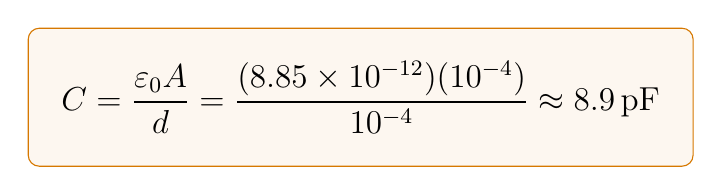
\begin{tikzpicture}
      \node[draw=cvolt, fill=cvolt!6, rounded corners=4pt, inner sep=12pt]
      {\large $\displaystyle C = \frac{\varepsilon_0 A}{d}
        = \frac{(8.85\times 10^{-12})(10^{-4})}{10^{-4}} \approx 8.9\uni{pF}$};
    \end{tikzpicture}
  \end{center}
  \vfill
  \begin{center}
    Which is why real values come in \alert{pF, nF and $\mu$F} ---\\
    and why a $1\uni{F}$ supercapacitor has to roll an enormous area into a small can.
  \end{center}
  \vfill
\end{frame}

%--------------------------------------------------------------
\begin{frame}{The LTI capacitor}
  \vfill
  \begin{center}
    {\large $\Qcol{q} = C\,\Vcol{v}$ \quad with $C$ constant. \quad Differentiate:}
  \end{center}
  \vfill
  \begin{center}
  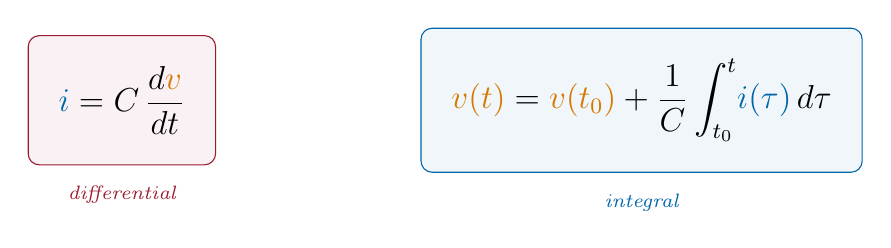
\begin{tikzpicture}[scale=1.0]
    \node[draw=metured, fill=metured!6, rounded corners=4pt, inner sep=11pt] (a) at (0,0)
      {\large $\displaystyle \Icol{i} = C\,\frac{d\Vcol{v}}{dt}$};
    \node[draw=ccur, fill=ccur!6, rounded corners=4pt, inner sep=11pt] (b) at (6.6,0)
      {\large $\displaystyle \Vcol{v(t)} = \Vcol{v(t_0)}
        + \frac{1}{C}\int_{t_0}^{t}\!\Icol{i(\tau)}\,d\tau$};
    \node[font=\scriptsize\itshape, text=metured, below=4pt of a] {differential};
    \node[font=\scriptsize\itshape, text=ccur, below=4pt of b] {integral};
  \end{tikzpicture}
  \end{center}
  \vfill
  \begin{center}
    The current is whatever the \alert{rate of change} of voltage demands.\\
    The voltage is the \alert{running total} of everything the current has done.
  \end{center}
  \vfill
\end{frame}

%--------------------------------------------------------------
\begin{frame}{Four consequences}
  \vfill
  \begin{columns}[T,onlytextwidth]
    \begin{column}{0.235\textwidth}
      \begin{block}{Open circuit at DC}
        \small $\Vcol{v}$ constant $\Rightarrow d\Vcol{v}/dt = 0 \Rightarrow \Icol{i}=0$.
      \end{block}
    \end{column}
    \begin{column}{0.235\textwidth}
      \begin{block}{Voltage cannot jump}
        \small Not with a finite current --- a step needs $d\Vcol{v}/dt = \infty$.
      \end{block}
    \end{column}
    \begin{column}{0.235\textwidth}
      \begin{block}{It remembers}
        \small $\Vcol{v(t)}$ depends on the \emph{whole history} of $\Icol{i}$.
      \end{block}
    \end{column}
    \begin{column}{0.235\textwidth}
      \begin{block}{It holds energy}
        \small $\Pcol{w} = \tfrac12 C\Vcol{v}^{\,2}$, set by the present voltage alone.
      \end{block}
    \end{column}
  \end{columns}
  \vfill
  \begin{center}
    {\large A resistor knows only \emph{now}, and keeps nothing.\\
     A capacitor knows everything that has happened to it --- and \alert{hands the energy
     back}.}
  \end{center}
  \vfill
\end{frame}

%--------------------------------------------------------------
\begin{frame}{Example: push a constant current in}
  \vfill
  \begin{center}
    $\Icol{I} = 1\uni{mA}$ into $C = 1\uni{\mu F}$, from $\Vcol{v(0)} = 0$
    \qquad
    \onslide<2->{$\displaystyle \Vcol{v(t)} = \frac{\Icol{I}}{C}\,t = 1000\,t$ \ [V]}
  \end{center}
  \vfill
  \begin{center}
  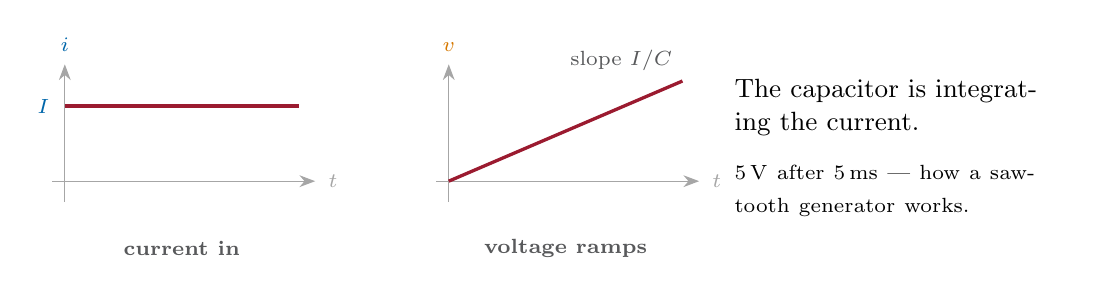
\begin{tikzpicture}[scale=1.06, transform shape]
    \begin{scope}
      \taxes{3.0}{0.25}{1.4}{\Icol{$i$}}
      \draw[crv] (0,0.9) -- (2.8,0.9);
      \node[font=\scriptsize, text=ccur, left] at (-0.06,0.9) {$I$};
      \node[ttl] at (1.4,-0.8) {current in};
    \end{scope}
    \begin{scope}[xshift=4.6cm]
      \taxes{3.0}{0.25}{1.4}{\Vcol{$v$}}
      \draw[crv, visible on=<2->] (0,0) -- (2.8,1.2);
      \node[font=\scriptsize, text=metugray, above left, visible on=<2->]
           at (2.8,1.2) {slope $I/C$};
      \node[ttl] at (1.4,-0.8) {voltage ramps};
    \end{scope}
    \node[font=\small, anchor=west, text width=3.9cm, visible on=<3->] at (7.9,0.4)
      {The capacitor is \alert{integrating} the current.\\[6pt]
       {\scriptsize $5\V$ after $5\uni{ms}$ --- how a sawtooth generator works.}};
  \end{tikzpicture}
  \end{center}
  \vfill
\end{frame}

%--------------------------------------------------------------
\begin{frame}{Example: hold the voltage constant}
  \vfill
  \begin{center}
    {\large $\Vcol{v} = V$ \ constant \quad$\Longrightarrow$\quad
     $\displaystyle \Icol{i} = C\,\frac{d\Vcol{v}}{dt} = 0$,
     \qquad $\Qcol{q} = CV$ \ sits there}
  \end{center}
  \vfill
  \begin{center}
    The capacitor has become an \alert{open circuit}, storing $CV$ while it does so.
  \end{center}
  \vfill
  \begin{center}
    {\large\color{metured} But how did the voltage get there?}
  \end{center}
  \vfill
\end{frame}

%--------------------------------------------------------------
\begin{frame}{A signal we have not met: the impulse}
  \vfill
  \begin{center}
  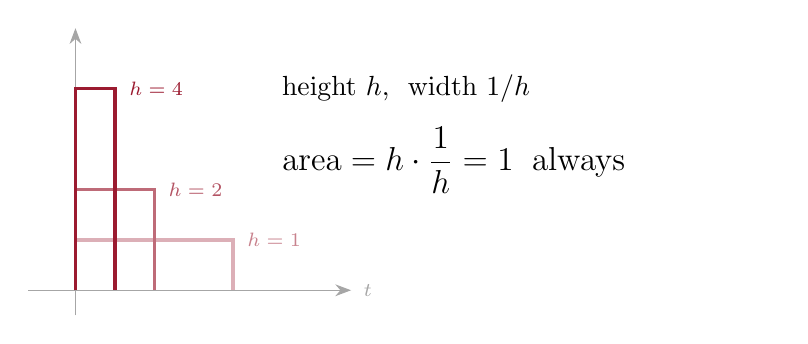
\begin{tikzpicture}[x=2.0cm, y=0.64cm]
    \draw[vax] (-0.3,0) -- (1.75,0) node[right=1pt, font=\scriptsize] {$t$};
    \draw[vax] (0,-0.5) -- (0,5.2);
    \draw[metured!35, very thick] (0,0) -- (0,1) -- (1.0,1) -- (1.0,0);
    \node[font=\scriptsize, text=metured!55, right] at (1.03,1) {$h = 1$};
    \draw[metured!65, very thick, visible on=<2->] (0,0) -- (0,2) -- (0.5,2) -- (0.5,0);
    \node[font=\scriptsize, text=metured!75, right, visible on=<2->] at (0.53,2) {$h = 2$};
    \draw[metured, very thick, visible on=<3->] (0,0) -- (0,4) -- (0.25,4) -- (0.25,0);
    \node[font=\scriptsize, text=metured, right, visible on=<3->] at (0.28,4) {$h = 4$};
    \node[font=\normalsize, anchor=west, text width=6.2cm] at (1.25,3.1)
      {height $h$, \ width $1/h$\\[8pt]
       {\large area $= h \cdot \dfrac{1}{h} = 1$ \ always}};
  \end{tikzpicture}
  \end{center}
  \vfill
  \begin{center}
    \onslide<4->{{\large Let $h$ grow: taller, narrower, \alert{the same area}.}\\[2pt]
      In the limit the width goes to zero and no value is left --- only the area.}
  \end{center}
  \vfill
\end{frame}

%--------------------------------------------------------------
\begin{frame}{The unit impulse $\delta(t)$}
  \vfill
  \begin{columns}[c,onlytextwidth]
    \begin{column}{0.36\textwidth}
      \begin{center}
      \begin{tikzpicture}[x=1.8cm, y=0.8cm]
        \draw[vax] (-0.3,0) -- (1.25,0) node[right=1pt, font=\scriptsize] {$t$};
        \draw[vax] (0,-0.35) -- (0,3.3);
        \draw[crv, very thick, -{Stealth[length=3.2mm]}] (0,0) -- (0,2.8);
        \node[font=\small, text=metured, right=4pt] at (0.04,2.45) {area $=1$};
        \node[ttl] at (0.5,-0.75) {$\delta(t)$};
      \end{tikzpicture}
      \end{center}
    \end{column}
    \begin{column}{0.60\textwidth}
      \begin{center}
        {\large $\delta(t) = 0$ for $t \neq 0$, \quad
         $\displaystyle\int_{a}^{b}\!\delta(\tau)\,d\tau = 1$}\\[4pt]
        {\small for any $a < 0 < b$}
      \end{center}
      \vspace{6pt}
      \begin{center}
        Not a function --- it is defined by its \alert{area}.\\[4pt]
        The number beside the arrow is its area, \alert{not a height}.\\[8pt]
        $K\,\delta(t)$ has area $K$.
      \end{center}
    \end{column}
  \end{columns}
  \vfill
  \begin{center}
    Two uses today: a current impulse $K\delta(t)$ delivers \alert{charge $K$} in zero
    time, and\\
    if $\Vcol{v}$ jumps by $V$ at $t=0$ then
    $\dfrac{d\Vcol{v}}{dt} = V\,\delta(t)$.
  \end{center}
  \vfill
\end{frame}

%--------------------------------------------------------------
\begin{frame}{The source steps from $0$ to $V$. What is the current?}
  \vspace{-0.1em}
  \begin{columns}[T,onlytextwidth]
    \begin{column}{0.48\textwidth}
      \begin{center}
      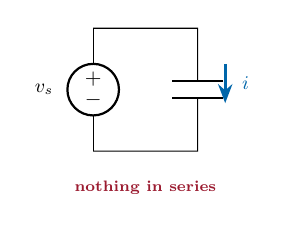
\begin{tikzpicture}[scale=0.78, transform shape]
        \draw (0,0) to[american voltage source, invert] (0,2.0);
        \draw (0,2.0) -- (1.7,2.0) to[C] (1.7,0) -- (0,0);
        \draw[iar] (2.15,1.42) -- (2.15,0.78);
        \node[ccur, font=\small] at (2.48,1.1) {$i$};
        \node[font=\small] at (-0.8,1.0) {$v_s$};
        \node[font=\scriptsize\bfseries, text=metured] at (0.85,-0.6) {nothing in series};
      \end{tikzpicture}
      \end{center}
      \vspace{2pt}
      \begin{center}
      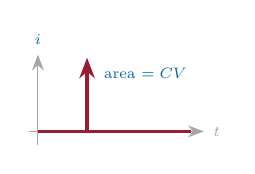
\begin{tikzpicture}[scale=0.78, transform shape]
        \taxes{2.7}{0.22}{1.25}{\Icol{$i$}}
        \draw[crv, visible on=<2->] (0,0) -- (0.8,0);
        \draw[crv, -{Stealth[length=2.6mm]}, visible on=<2->] (0.8,0) -- (0.8,1.2);
        \draw[crv, visible on=<2->] (0.8,0) -- (2.5,0);
        \node[font=\scriptsize, text=ccur, right=2pt, visible on=<2->]
             at (0.88,0.95) {area $= CV$};
      \end{tikzpicture}
      \end{center}
    \end{column}
    \begin{column}{0.48\textwidth}
      \begin{center}
      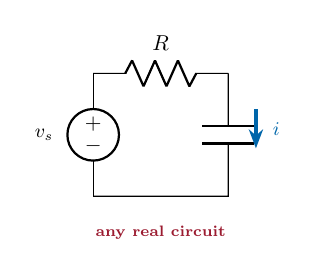
\begin{tikzpicture}[scale=0.78, transform shape]
        \draw (0,0) to[american voltage source, invert] (0,2.0);
        \draw (0,2.0) to[R, l=$R$] (2.2,2.0);
        \draw (2.2,2.0) to[C] (2.2,0) -- (0,0);
        \draw[iar] (2.65,1.42) -- (2.65,0.78);
        \node[ccur, font=\small] at (2.98,1.1) {$i$};
        \node[font=\small] at (-0.8,1.0) {$v_s$};
        \node[font=\scriptsize\bfseries, text=metured] at (1.1,-0.6) {any real circuit};
      \end{tikzpicture}
      \end{center}
      \vspace{2pt}
      \begin{center}
      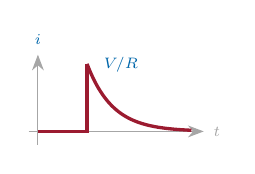
\begin{tikzpicture}[scale=0.78, transform shape]
        \taxes{2.7}{0.22}{1.25}{\Icol{$i$}}
        \draw[crv, domain=0:1.7, samples=95, smooth, visible on=<3->]
             plot ({0.8+\x}, {1.1*exp(-2.4*\x)});
        \draw[crv, visible on=<3->] (0,0) -- (0.8,0) -- (0.8,1.1);
        \node[font=\scriptsize, text=ccur, right=2pt, visible on=<3->]
             at (0.88,1.08) {$V/R$};
      \end{tikzpicture}
      \end{center}
    \end{column}
  \end{columns}
  \vspace{0.2em}
  \begin{center}\footnotesize
    \onslide<2->{Differentiate the step:
      $\Icol{i} = C\,d\Vcol{v}/dt = CV\,\delta(t)$ --- an \alert{impulse} of area
      $CV$.\\[2pt]}
    \onslide<3->{With $R$ there the current starts at $V/R$ and decays while $\Vcol{v}$
      rises smoothly to $V$ --- \alert{we will solve this circuit in detail later}.}
  \end{center}
\end{frame}

%--------------------------------------------------------------
\begin{frame}{Example: read a current waveform}
  \vfill
  \begin{center}
  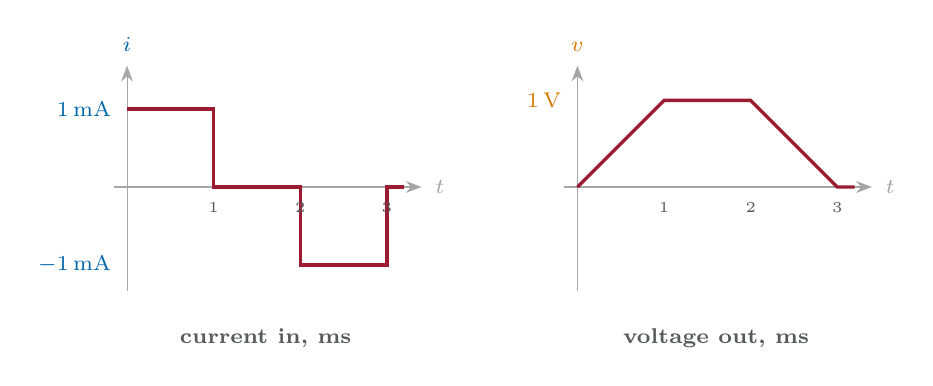
\begin{tikzpicture}[scale=1.1, transform shape]
    \begin{scope}
      \taxes{3.4}{1.2}{1.4}{\Icol{$i$}}
      \draw[crv] (0,0.9) -- (1.0,0.9) -- (1.0,0) -- (2.0,0) -- (2.0,-0.9) -- (3.0,-0.9)
                 -- (3.0,0) -- (3.2,0);
      \node[font=\scriptsize, text=ccur, left] at (-0.06,0.9) {$1\uni{mA}$};
      \node[font=\scriptsize, text=ccur, left] at (-0.06,-0.9) {$-1\uni{mA}$};
      \foreach \x/\lb in {1.0/{1}, 2.0/{2}, 3.0/{3}}{
        \node[font=\tiny, text=metugray, below] at (\x,-0.06) {\lb};}
      \node[ttl] at (1.6,-1.75) {current in, ms};
    \end{scope}
    \begin{scope}[xshift=5.2cm]
      \taxes{3.4}{1.2}{1.4}{\Vcol{$v$}}
      \draw[crv, visible on=<2->] (0,0) -- (1.0,1.0) -- (2.0,1.0) -- (3.0,0) -- (3.2,0);
      \node[font=\scriptsize, text=cvolt, left, visible on=<2->] at (-0.06,1.0) {$1\V$};
      \foreach \x/\lb in {1.0/{1}, 2.0/{2}, 3.0/{3}}{
        \node[font=\tiny, text=metugray, below] at (\x,-0.06) {\lb};}
      \node[ttl] at (1.6,-1.75) {voltage out, ms};
    \end{scope}
  \end{tikzpicture}
  \end{center}
  \vfill
  \begin{center}
    \onslide<2->{Constant current $\Rightarrow$ straight line, slope $\Icol{i}/C$. \
    Zero current $\Rightarrow$ the voltage holds.\\[4pt]}
    \onslide<3->{It ends where it started, having given back exactly the charge it took.}
  \end{center}
  \vfill
\end{frame}

%--------------------------------------------------------------
\begin{frame}{Energy stored in a capacitor}
  \vfill
  \begin{center}
    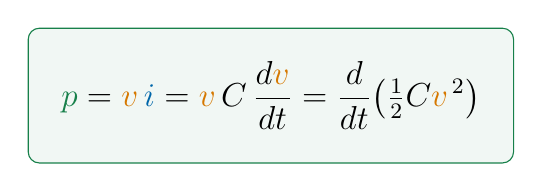
\begin{tikzpicture}
      \node[draw=cpow, fill=cpow!6, rounded corners=4pt, inner sep=12pt]
      {\large $\displaystyle \Pcol{p} = \Vcol{v}\,\Icol{i}
        = \Vcol{v}\,C\,\frac{d\Vcol{v}}{dt}
        = \frac{d}{dt}\!\left(\tfrac12 C \Vcol{v}^{\,2}\right)$};
    \end{tikzpicture}
  \end{center}
  \vfill
  \begin{center}
    {\large The power is the \alert{rate of change} of $\tfrac12 C \Vcol{v}^{\,2}$.\\
     So that is the energy the capacitor holds:}
  \end{center}
  \vfill
  \begin{center}
    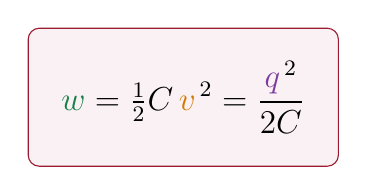
\begin{tikzpicture}
      \node[draw=metured, fill=metured!6, rounded corners=4pt, inner sep=12pt]
      {\large $\displaystyle \Pcol{w} = \tfrac12 C\,\Vcol{v}^{\,2}
        = \frac{\Qcol{q}^{\,2}}{2C}$};
    \end{tikzpicture}
  \end{center}
  \vfill
  \begin{center}
    It depends only on the \alert{present} voltage --- not on how the capacitor got there.
  \end{center}
  \vfill
\end{frame}

%--------------------------------------------------------------
\begin{frame}{Resistor and capacitor, side by side}
  \vfill
  \begin{center}
  \renewcommand{\arraystretch}{1.3}
  \begin{tabular}{@{}l l l@{}}
    \toprule
     & \textbf{LTI resistor} {\footnotesize(Lecture 3)} & \textbf{LTI capacitor}\\
    \midrule
    terminal equation & $\Vcol{v} = R\Icol{i}$ & $\Icol{i} = C\,d\Vcol{v}/dt$\\
    plane it lives in & $\Vcol{v}$--$\Icol{i}$ & $\Vcol{v}$--$\Qcol{q}$\\
    memory            & none & the whole past of $\Icol{i}$\\
    power             & $R\Icol{i}^2 \ge 0$ always & either sign\\
    energy            & dissipated as heat, gone & stored, all of it returnable\\
    verdict           & passive, \alert{lossy} & passive, \alert{lossless}\\
    \bottomrule
  \end{tabular}
  \end{center}
  \vfill
\end{frame}

%--------------------------------------------------------------
\begin{frame}{For the mechanically minded}
  \vfill
  \begin{center}
    {\Large $\displaystyle \Icol{i} = C\,\frac{d\Vcol{v}}{dt}
      \qquad\longleftrightarrow\qquad F = m\,\frac{du}{dt}$}
  \end{center}
  \vfill
  \begin{center}
  \begin{tabular}{@{}c c c@{}}
    \toprule
    \textbf{electrical} & & \textbf{mechanical}\\
    \midrule
    \Icol{current $i$}  & $\leftrightarrow$ & force $F$\\
    \Vcol{voltage $v$}  & $\leftrightarrow$ & velocity $u$\\
    capacitance $C$     & $\leftrightarrow$ & mass $m$\\
    $\tfrac12 C\Vcol{v}^{\,2}$ & $\leftrightarrow$ & $\tfrac12 m u^2$\\
    \bottomrule
  \end{tabular}
  \end{center}
  \vfill
  \begin{center}
    {\large A heavy flywheel is a large capacitance.}\\[6pt]
    A finite force cannot change its speed instantly ---\\
    and a finite current cannot change a capacitor's voltage instantly.
  \end{center}
  \vfill
\end{frame}

%--------------------------------------------------------------
\begin{frame}{Summary}
  \vfill
  \begin{itemize}\itemsep5pt
    \item An \textbf{ideal energy-storage element}: it dissipates nothing, and everything
          put in can be taken back out. Lecture~3's elements dissipated all of it.
    \item A \textbf{capacitor} is a curve in the $\Vcol{v}$--$\Qcol{q}$ plane, not a
          resistor --- no $f$ with $\Icol{i(t)} = f(\Vcol{v(t)})$.
    \item $C = \varepsilon A/d$, in farads. One farad is enormous; real values are pF, nF,
          $\mu$F.
    \item \textbf{LTI capacitor}: $\Icol{i} = C\,d\Vcol{v}/dt$, or the integral form.
          Open circuit at DC; voltage cannot jump; it remembers.
    \item $\Pcol{w} = \tfrac12 C\Vcol{v}^2 = \Qcol{q}^2/2C$ --- stored, not spent; set by
          the present voltage alone. Passive and \alert{lossless}.
  \end{itemize}
  \vfill
\end{frame}

%--------------------------------------------------------------
\begin{frame}{Next lecture}
  \vfill
  \begin{center}
  \begin{block}{The inductor}
    The \emph{second} ideal energy-storage element, and the mirror image of today:
    flux linkage and current in place of charge and voltage,
    $\tfrac12 L\Icol{i}^2$ in place of $\tfrac12 C\Vcol{v}^2$.
  \end{block}
  \end{center}
  \vfill
  \begin{center}
    {\Large\color{metured} Questions?}\\[8pt]
    {\small Notes for this lecture: see the course repository.}
  \end{center}
  \vfill
\end{frame}

\end{document}
